
\documentclass[12pt]{article}



%% The amssymb package provides various useful mathematical symbols
\usepackage{amssymb}
%% The amsmath package provides various useful equation environments.
\usepackage{amsmath}
%% The amsthm package provides extended theorem environments
%% \usepackage{amsthm}

\usepackage{setspace}
\usepackage{xcolor}

\usepackage{placeins}
% \usepackage{amsmath}
\usepackage{bm}
% \usepackage{amssymb}
\usepackage[nopatch]{microtype}
\usepackage{booktabs}
\usepackage{mathtools} % Loads amsmath
\usepackage{setspace}
\usepackage{hyperref}


\usepackage[authoryear]{natbib}
\setcitestyle{aysep={}} 

% \bibliography{example}
% \bibliographystyle{elsarticle-harv}

\begin{document}



\title{An Election Forecasting Model for Subnational Elections} %% Article title

%% use optional labels to link authors explicitly to addresses:
%% \author[label1,label2]{}
%% \affiliation[label1]{organization={},
%%             addressline={},
%%             city={},
%%             postcode={},
%%             state={},
%%             country={}}
%%
%% \affiliation[label2]{organization={},
%%             addressline={},
%%             city={},
%%             postcode={},
%%             state={},
%%             country={}}

\author{} %% Author name
\maketitle


%% Abstract
\begin{abstract}
%% Text of abstract
While election forecasts predominantly focus on national contests, many democratic elections take place at the subnational level.  Subnational elections pose unique challenges for traditional fundamentals forecasting models due to less available polling data and idiosyncratic subnational politics. In this article, we present and evaluate the performance of Bayesian forecasting models for German state elections from 1990 to 2024. Our forecasts demonstrate high accuracy at lead times of two days, two weeks, and two months, and offer valuable ex-ante predictions for three state elections held in September 2024. These findings underscore the potential for applying election forecasting models effectively to subnational elections.
\end{abstract}





\section{Introduction}


\begin{doublespacing}


Although many democratic elections take place at the subnational level, academic election forecasting has predominantly focused on national elections~\citep[see e.g.][]{lewis2005election,stegmaier2022forecasting,stegmaier2023evolution}. The outcomes of subnational elections are significant for democratic satisfaction~\citep{singh2012differentiating}, shape local policies~\citep{alt2000dynamic,uppal2011does}, and often serve as indicators of broader national trends, such as the rise of antidemocratic parties~\citep{arzheimer2019don}. In this sense, state elections have also been used to predict national-level elections~\citep{kayser2017lander} or explain state-level support at national elections~\citep{erikson2015gubernatorial}. \textcolor{red}{However, while they are often analyzed in the national context to identify broader political shifts, dedicated forecasting models for subnational elections remain rare. Developing such models not only provides insights into subnational political dynamics but also helps evaluate the reliability of forecasting approaches and their theoretical and methodological foundations beyond national contexts.}

\textcolor{red}{Forecasting subnational elections presents unique challenges for traditional election forecasting models, which typically depend on pre-election polls or fundamental variables—such as economic indicators, incumbency status, and government approval ratings—to predict electoral outcomes \citep{lewis2015forecasting,nadeau2020election}.} At the subnational level, pre-election polls are often scarce, making it difficult to average out common polling errors. For fundamentals-based models, the challenge lies in the variability of elections between subnational units, including differences in the competing parties, which may not always allow for the identification of comparable and stable patterns. However, subnational elections present a distinct opportunity: the consistent participation of similar parties across various units under comparable electoral systems allows for the pooling of information across elections.

In this paper, we develop a new Bayesian election forecasting model and evaluate its applicability to subnational elections. Our model integrates a dynamic analysis of subnational election polls with fundamental predictors and is applied to German state elections from 1990 to 2024. \textcolor{red}{It addresses key challenges by incorporating a dynamic polling model that enables the interpolation of latent support before the election even in contexts with sparse polling data. Additionally, by structuring the model at the party-election level, we account for variability across elections with different party compositions while still identifying stable patterns.} Compared to forecasting models that rely solely on polls, the inclusion of fundamentals improves performance, particularly when forecasting elections further in advance. Using a Bayesian framework allows us to quantify key uncertainties, such as the probabilities of various coalition majorities forming.

We evaluate the model using two approaches. First, we assess its out-of-sample performance in German state elections since 2010, finding that it performed satisfactorily. Notably, the combination of polls and fundamentals proves to be particularly effective and comes with a mean absolute error (MAE) of 1.46 percentage points (pp) with a lead time of two days, of 2.16~pp with a lead time of two weeks, and an MAE of 3.09~pp with a lead time of two months.  Second, we present preregistered ex-ante forecasts for three state elections held in September 2024. The forecasts performed well, with an MAE of 3.16~pp across all elections and parties two months prior to the elections. The election results fell within credible intervals and the model provided useful forecasts even for a newly emerging party. Importantly, both evaluation exercises show that election forecasting models for subnational elections are on par with comparable national election forecasts~\citep{jennings2018election,shirani2018disentangling,munzert_2017}.

Our paper makes a significant contribution to the election forecasting literature by demonstrating that forecasting models can be successfully applied to subnational elections. Additionally, we present a general and flexible Bayesian forecasting model for multiparty elections that integrates information from polls and fundamentals. This model can be applied to other subnational contexts and also national elections, and serve as a foundation for further refinements of general election forecasting models.

\section{\textcolor{red}{Literature Review}}

Forecasting election outcomes has a long tradition in political science, with various approaches having been developed over the years. These models are broadly categorized into fundamentals-based models, poll-based models, and synthetic approaches that combine various different methods.

% \paragraph{Fundamentals Models}
Fundamentals-based models primarily rely on structural variables that influence election outcomes over time, such as economic indicators, incumbency status, party strength, and long-term political trends. A prominent example is the work by \citet{hummel2014fundamental}, which emphasizes non-polling predictors like past election results, economic conditions, presidential approval, and other characteristics. These models aim to capture the underlying conditions that shape voter preferences long before the election season, enabling early forecasting.

% \paragraph{Poll-based Forecasts}
Poll-based models, also referred to as poll-aggregation models, focus on opinion polling data collected closer to the election date. These models have become increasingly sophisticated by incorporating adjustments for sampling error, non-response bias, and methodological differences between polling organizations, so-called house effects~\citep{shirani2018disentangling,jackman2005pooling}. Poll-based forecasts tend to increase in accuracy as the election date approaches, as they reflect the most recent distribution of voter intentions.

% \paragraph{Combined Approaches}
A third category of models combines the strengths of fundamentals and poll-based approaches in synthetic forecasting models\citep{Lewis-Beck_Nadeau_Belanger_2016, Lewis-Beck_Dassonneville_2015}. By integrating structural fundamentals with polling data, these models seek to offer more robust forecasts that balance the long-term stability of fundamentals with the short-term precision provided by polls~\citep{munzert_2017}. For example, \citet{MONTALVO201952} developed a hybrid model that incorporates new parties and focuses on predicting parliamentary seat distributions. Other hybrid models have been proposed for forecasting German national elections~\citep{Stoetzer_Neunhoeffer_Gschwend_Munzert_Sternberg_2019} and US Senate elections~\citep{Chen_Garnett_Montgomery_2023}.

% \paragraph{Limited Application to Subnational Elections}
Although these forecasting models have proven successful at the national level, their application to subnational elections has been more limited. Forecasting subnational elections—such as state or regional contests—presents additional challenges due to smaller sample sizes, localized issues, and greater variability in electoral behavior across regions. Additionally, subnational elections often involve a larger number of parties, with new parties appearing more frequently, increasing model complexity.  Some efforts have been made to forecast national election outcomes at the district level in Germany~\citep{munzert2017forecasting, neunhoeffer2020ansatz}, and to predict by-election outcomes using national-level polling data~\citep{hanretty2021forecasting}. Similarly, district-level outcomes of U.S. presidential and U.K. general elections have been modeled~\citep{LAUDERDALE2020399}. 

\color{red}
Several studies have developed structural models for forecasting subnational elections in the U.S. For example, \citet{bardwell2004state} presents a state-level model for forecasting U.S. Senate elections, while \citet{linzer2013dynamic} applies a Bayesian approach to predict U.S. presidential election outcomes at the state level. Similarly, \citet{klarner2010forecasting, klarner20182018} introduce models for forecasting U.S. state legislative elections in 2010 and 2018, respectively. In the context of gubernatorial races, \citet{hummel2014fundamental} develops a model accounting for state-level fundamentals.
\color{black}


\section{A Forecasting Model for Subnational Elections}

In this section, we develop a forecasting model for subnational elections. \textcolor{red}{Our model follows a synthetic forecasting framework, integrating both fundamental and polling-based predictors \citep{Lewis-Beck_Nadeau_Belanger_2016, Lewis-Beck_Dassonneville_2015}.}

 \textcolor{red}{The target for our forecasting model are subnational election results.} We assume that each observation \( v_i \), where $i = (k,e) \in \mathcal{K} \times \mathcal{E}$, represents the vote share of a party $k \in \mathcal{K} $   in a subnational election $e \in \mathcal{E}$.\footnote{The vote shares fall into the unit interval \( 0 < v_i < 1 \). Additionally, the vote shares of all parties in any given election sum to one, i.e., $\sum v_i = 1$.} In applications, we select a number of relevant parties $k_j \in \mathcal{K}$ for each election $e$ and subsume all other parties into a residual party $k_{res} \in \mathcal{K}$ called `Others'.

 \textcolor{red}{To build the polls-based part of our forecasting model}, we have data from pre-election polls \( p_{i,t} \), i.e., we have the share of voters in a poll published \textit{before} election $e$ that intend to vote for each party $k$. Since these vote shares potentially vary across each day $t \in \{1, \ldots, T_e\}$ between the previous and the upcoming election $e$, we collect all poll data for all parties  before a subnational election $e$ in a row vector \( \boldsymbol{p}_{i} = (p_{i,1}, \ldots, p_{i,T_{e}}) \) of length $T_e$.   Each entry \( p_{i,t} \) represents the published poll-based vote shares for party $k$ in election $e$ if a poll was published on day \( t \), or  is set to missing otherwise. We further define the lead time at time $t$ to election  $e$ as $l = T_{e} - t$ with $l \in \{1, \ldots, T_e\}$.
 
\textcolor{red}{We first devise a dynamic model to estimate the latent support for party \( k \)  prior to an election \( e \), based on polling data. To do so, we employ a \textit{dynamic linear model} with a random walk component~\citep{west1997}.\footnote{Most poll dynamic models rely on dynamic linear models~\citep{walther2015picking} or apply transformations to adapt poll data to continuous measurement error assumptions~\citep{Stoetzer_Neunhoeffer_Gschwend_Munzert_Sternberg_2019}. For an alternative approach using non-linear state space models for polling data, see~\citep{stoetzer2020estimating}.} The dynamic model consists of two key components: a \textit{measurement equation}, which links observed polling data to the unobserved latent support, and a \textit{latent state equation}, which describes how latent support evolves over time.}

\textcolor{red}{The \textit{measurement equation} is specified as follows:}

\begin{equation}
p_{i,t} = \pi_{i,t} + \epsilon_{i,t}, \quad \epsilon_{i,t} \sim \mathcal{N}(0, R_{i})
\end{equation}

\textcolor{red}{This equation states that the observed poll share \( p_{i,t} \) for the parties at time \( t \) consists of the latent true support \( \pi_{i,t} \) plus an observation error term \( \epsilon_{i,t} \), which is assumed to be normally distributed with variance \( R_i \). The term \( R_i \) reflects the uncertainty in individual polls, accounting for sampling variability and other sources of measurement error.}

\textcolor{red}{The \textit{latent state equation}, which governs the temporal evolution of latent party support, is defined as:}

\begin{equation}
\pi_{i,t} = \pi_{i,t-1} + \eta_{i,t}, \quad \eta_{i,t} \sim \mathcal{N}(0, Q_{i})
\end{equation}

\textcolor{red}{Here, the latent party support \( \pi_{i,t} \) follows a \textit{random walk}, meaning that the best predictor for current support is simply the previous period’s party support plus a stochastic evolution term \( \eta_{i,t} \). This formulation assumes that changes in support occur incrementally over time rather than experiencing sudden jumps, making it well-suited for modeling gradual shifts in voter support. The variance \( Q_i \) captures the degree of expected change in latent support over time and is specific to each party-election combination. To initialize the process, we assume an initial latent state: $\pi_{i,0} \sim \mathcal{N}(m_0, S_0)
$, where \( m_0 \) represents the prior expectation of support before polling data is observed, and \( S_0 \) represents the initial uncertainty.}

\textcolor{red}{This framework allows us to estimate the latent support for each party before a subnational election over time}, accounting for both the random evolution of actual support and the inherent noise in poll data. For estimation, we only use data up to a specific lead time $l$ to  election $e$,  such that we only consider polls that were published up to $l$ days prior to that election. This subsets the data for each party to \( \boldsymbol{p}_{i} = (p_{i,1},  \ldots, p_{i,T_{e}-l})\), a vector of length $T_{e}-l$. Given a specific lead time, we estimate the latent support using a Kalman filter~\citep[][p.103-107]{west1997}.\footnote{We estimate the model variances (observational error variance and evolution variance) using maximum likelihood routine and set uninformative priors on the initial latent states ($m_0 = 0$, $S_0 = 5$). The estimation is implemented using the R-package dlm~\citep{petris2010dlm}.} The advantage of using a dynamic linear model is that it provides latent support estimates for all lead times before an election, even if no polls were published on that day or within a nearby time-frame. This allows us to relate the latent support for a party to the election result at different lead times.\footnote{If there are no polls available for a particular party at a specific lead time before the election, we cannot estimate the dynamic linear model, and the latent support for this party is marked as missing} 

\textcolor{red}{Next, we integrate the poll-based with the fundamentals-based model to forecast the election results.} We assume that the vote share of a party $v_i$ is related to a set of observed fundamental predictors, and the latent support from the dynamic linear model with a specific lead time. \textcolor{red}{The fundamental predictor variables are factors theoretically related to the support of political parties in upcoming elections, such as economic indicators, incumbency status, and government approval ratings.}\footnote{\textcolor{red}{It is important to note that we define a general framework rather than pre-specifying a fixed set of fundamental predictors. The relevant predictors will vary depending on the specific application. For our application to German state elections, for example, we select predictors with a strong theoretical foundation in political science debates on voting behavior in Germany.}} We collect these observed fundamentals predictors in a matrix $\bm{X}$ that has $N$ rows and the $C$ predictors in respective columns.  
$\bm{x}_i$ is a row vector that holds the values of all the $C$ predictors of $v_i$, the vote share of party $k$ in an election $e$. In order to identify a constant term for the systematic component of the model, we add a column with ones to the $C$ predictors in matrix $\bm{X}$. The latent support ${\pi}_{i,l}$ for party $k$ before election $e$ with a specific lead time $l$ is taken from the dynamic linear model that is estimated based on data available at this lead time. We collect the support for all parties before election $e$ with a given lead time in a column vector $\bm{\pi}_{l}$. %To take into account the constraint that all vote shares sum-up to $1$, 

\textcolor{red}{To ensure that our vote share forecasts remain within the 0\% to 100\% range, we apply a transformation to the dependent variable.}  We use a log ratio transformation for the observed election outcomes $\hat{v}_i = \ln{\frac{v_i}{1-v_i}}$ to ensure that estimated confidence intervals for the untransformed election outcomes fall within the unit interval.  The linear regression model with log ratio transformed vote shares is defined as:

\begin{eqnarray}
        \hat{v}_i &\sim& N\left(\mu_i, \sigma \right) \\
        \mu_i & =& \boldsymbol{x_i} \boldsymbol{\beta}' + \gamma {\pi}_{i,l}
\end{eqnarray}

where $\boldsymbol{\beta}$ are the effects of the fundamental predictor variables including the constant, $\gamma$ the effect of ${\pi}_{i,l}$, the latent support for the parties  with an election-specific lead time $l$, and the constant error variance $\sigma$. \textcolor{red}{The effect parameters indicate how the expected log-ratio vote shares changes with a change in the fundamental predictor variables or the latent support in the polls.} We collect the parameters of the model in a vector $\bm{\theta}  = [\bm{\beta},\gamma,\sigma]$. 

We estimate the model using Bayesian methods.\footnote{\textcolor{red}{We employ Bayesian estimation for its intuitive probabilistic interpretation of credibility intervals, which allows direct probability statements about events—unlike conventional confidence intervals. This approach is particularly effective in communicating uncertainty to a general audience. For instance, we report 5/6 credible intervals, meaning that the vote share of each party has a 5-in-6 probability of falling within this range—akin to rolling any number except a six on a fair dice. This enhances interpretability and facilitates communication, as demonstrated in recent Bayesian election forecasts \citep{Stoetzer_Neunhoeffer_Gschwend_Munzert_Sternberg_2019, Kang2024forecasting, Chen2023polls}.}} The posterior distribution of the model parameters is proportional to the likelihood times the priors, while $\boldsymbol{X}$ and $\boldsymbol{\pi}_{l}$ is fixed in the likelihood  and $\bm{v}$ is the vector of vote shares. 

\begin{equation}
    P\left(\bm{\theta} \mid \bm{v},  \bm{X},  \bm{\pi}_{l} \right) \propto  P\left(\bm{v} \mid \bm{\theta},\bm{X},  \bm{\pi}_{l}\right) P\left(\bm{\theta}\right)
\end{equation}

\textcolor{red}{Bayesian estimation requires the specification of priors  beliefs about the parameters of the model}. The priors are defined in terms of a probability distribution $P\left(\bm{\theta}\right)$. We generally assume pairwise independent distributions for $P\left(\bm{\theta}\right) \propto P\left(\bm{\beta}\right)P\left( \gamma\right)P\left(\sigma \right)$ and use application-specific priors.

\textcolor{red}{Based on the model, we can obtain a forecast for the upcoming election.} We define the predicted vote shares for the relevant parties in the upcoming election as $\bm{v}^{\star}$ (excluding party $k_{res}$)\footnote{For the forecasts, we leave out the support for parties in the residual category $k_{res}$. This implies that the remaining vote share for these other parties is set to the rest when the predicted vote shares of the relevant parties is subtracted from 100\%.}, $\bm{X}^{\star}$ holds the values of the fundamental predictor variables, and $\bm{\pi}_{l}^{\star}$ represents the estimated  latent support of the parties given a specific lead time. With this, we can compute the posterior predictive distribution. 


\begin{equation}
P\left(\bm{v}^{\star} \mid \bm{X}^{\star}, \bm{\pi}_{l}^{\star} \right) = \int_{\bm{\theta}} P\left(\bm{v}^{\star} \mid \bm{X}^{\star},  \bm{\pi}_{l}^{\star},  \bm{\theta} \right)  P\left(\bm{\theta} \mid \bm{v}, \bm{X},  \bm{\pi}_{l}  \right) d\bm{\theta}.
\end{equation}

\textcolor{red}{The posterior predictive distribution represents the probability distribution of future vote shares given new predictor values, incorporating the uncertainty in our parameter estimates. It is obtained by integrating over the posterior distribution of the parameters, effectively averaging predictions across all plausible parameter values inferred from the observed data.}

\textcolor{red}{The posterior predictive distribution allows us to generate forecasts from the model. We can derive point estimates for election results using the posterior mean and construct credible intervals to quantify the inherent uncertainty in our predictions}. 
%$\mathbb{E} [ P\left(\bm{v}^{\star} \mid \bm{X}^{\star}, \bm{\pi}_{l}^{\star} \right) ]$, 
 

\textcolor{red}{To implement the estimation and forecasting, we rely on Markov Chain Monte Carlo (MCMC) methods}. We sample from the posterior distribution and the posterior predictive distribution to obtain forecasts for upcoming elections using the No-U-Turn sampler (NUTS)~\citep{carpenter2017stan} as implemented in Stan, which we access using the R-package rstanarm~\citep{rstanarm}.  

\section{\textcolor{red}{The Case of German State Elections}}

% \section{Application to German State Elections}

We apply our model to subnational elections in Germany, a federal country with 16 states and corresponding state parliaments.  The electoral systems in these 16 states are comparable, with most of them being characterized by the federal mixed-member proportional system, which strongly focuses on party lists. The party systems are also comparable, with most major parties competing in all state elections: CDU/CSU, SPD, FDP, Greens, Die Linke (formerly PDS), and AfD. One exception is the CSU, which only competes in Bavaria, while the CDU competes in the remaining 15 states. In our ex-ante forecasts for the September 2024 state elections, we include the BSW, a newly formed party composed of former Die Linke members.\footnote{We decided to also produce forecasts for the newly formed BSW as it has quickly gained national significance and also polled above 10\% in the state elections. Its rapid rise in the polls makes it a critical player to consider. }
% Cornelius:

% Selection of parties
We leverage the overall cohesiveness and comparable voter perceptions across state-level chapters of a party to generalize findings, even though minor policy differences exist between chapters of the same party~\citep{Brauninger2020}. This cross-state comparison strengthens our model by expanding its empirical foundation and improving its predictive accuracy through the identification of systemic patterns. One key strength of our model is its flexibility to include emerging or new parties as needed. However, in past elections, we have focused on parties with a presence in most German states to ensure polling data availability, which is essential for applying our combined model.\footnote{Some smaller parties have gained substantial vote shares in certain state elections and are included in polling data. However, we focus on the major parties, grouping these smaller parties in a residual category (`Other'), as they are not central to the ex-ante forecasts in this paper. Our model also implicitly accounts for excluded parties by calculating their combined vote share as the remainder after subtracting the vote shares of the modeled parties. This approach ensures that all parties, even those not explicitly modeled, are considered in the analysis.}
% BSW


% Other category


% We could have included FW in Brandenburg, but ?

%%%%%%%%%%%%%%%%%%%%%%%%%%%%%%%%%%%%%%%%%%%%%%%%%%%%%%%%%%%%
%%%%%%%%%%%%%%% TODO %%%%%%%%%%%%%%%%%%%%%%%%%%%%%%%%%%%%%%%
%%%%%%%%%%%%%%%%%%%%%%%%%%%%%%%%%%%%%%%%%%%%%%%%%%%%%%%%%%%%

% - [ ] Address the variability of party systems:
%   - Discuss the implications of AfD’s resurgence, BSW’s formation, and FW’s role in Bavaria.
%   - Explain why aggregating across all state elections is justified despite variability.
% - [ ] Incorporate an indicator for each Bundesland into the model.

% - [ ] Define and justify the selection of "relevant" parties:
%   - Address how you determine relevant parties (e.g., Sartori’s effective parties).
%   - Justify why “usual suspects” are chosen despite the complexity of subnational elections. (model learns from pooling across states)
%   - Clarify the issues with BSW and how information about “unusual” parties is managed.
% - [ ] Revisit the “Other” category for parties:
%   - Explain why parties in “Other” are considered irrelevant or justify why they are excluded.

\autoref{fig:polls_results} shows both,  election and polling results for major parties in the state of Brandenburg over time. Graphs for the remaining 15 German states can be found in SM~A. While patterns vary across states, continuously progressing party system fragmentation is an evident general trend. Founded in 2013, the AfD entered all state parliaments by 2016. The BSW, founded in 2024, first participated in the 2024 European elections and subsequently secured seats in the state parliaments of all three states analyzed here. % Many different patterns


\begin{figure}[!t]
    \centering
    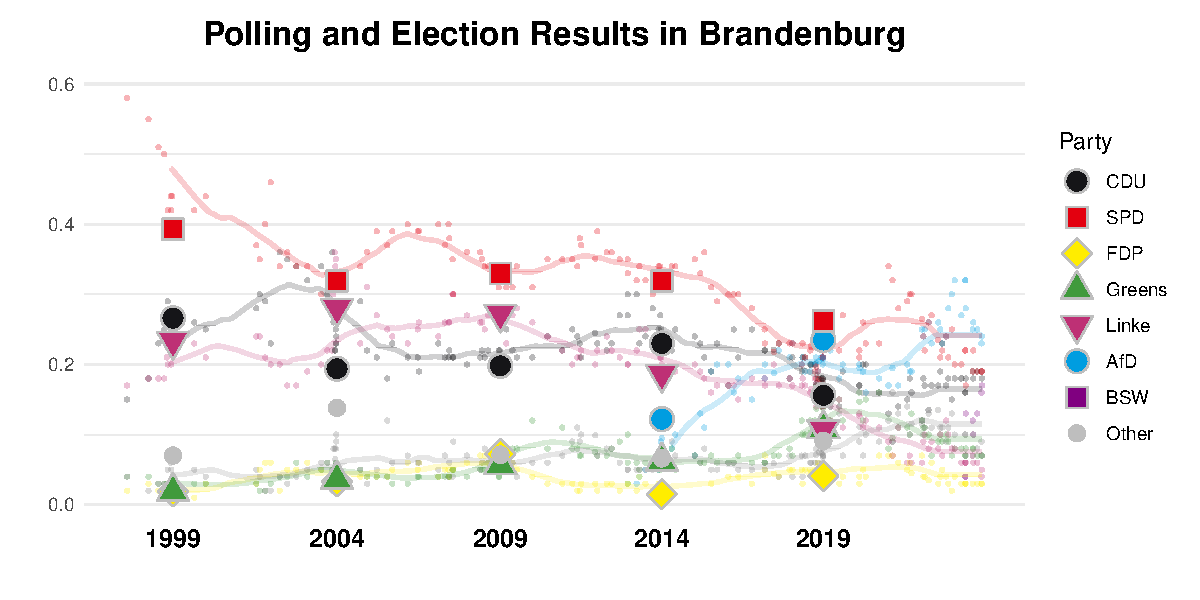
\includegraphics[width=\textwidth]{fg1_fig_poll_bb.pdf}  
    \caption{Polls and election results over time in Brandenburg. The symbols show the election results. The small dots show polling results between elections. The lines are 1000 day rolling averages of the polls.}
    \label{fig:polls_results}
\end{figure}

We collected polling data for state elections from various sources. \autoref{fig:polls-coverage} illustrates all state elections since 1946 and the coverage of election polls. \textcolor{red}{The grey diamonds represent election dates and the black rectangular sections indicate available polling data. The larger the rectangles, the more polling data is available for a time segment.}
We accessed published polling data from \citet{dawum_state_polls} and \citet{wahlrecht_state_polls}. The dataset comprises 2,857 state-level polls since 1993, covering 98 of 247 state elections since 1946\footnote{This includes the states of the former German Democratic Republic after reunification in 1990.}. The polls come from approximately 10 major and 50 smaller polling organizations. The number of available polls has consistently increased, with more than 200 polls per year from 2001 onward and over 1,000 polls in 2022 and 2023. For the forecasting effort we report here, we also conducted two surveys in Saxony preceding the 2024 state election, each with about 950 respondents; the responses were raked before being incorporated into our forecast. Given the often limited number of available polls, we choose to incorporate data from all polling providers. Potential polling errors are accounted for by our model through the incorporation of uncertainty. 
When a larger set of polls becomes available, any individual survey biases are mitigated by averaging results across multiple sources. The  performance of our model, \textcolor{red}{as described in section 5.2}, demonstrates that this approach works well for our application.


%%%%%%%%%%%%%%%%%%%%%%%%%%%%%%%%%%%%%%%%%%%%%%%%%%%%%%%%%%%%
%%%%%%%%%%%%%%% TODO %%%%%%%%%%%%%%%%%%%%%%%%%%%%%%%%%%%%%%%
%%%%%%%%%%%%%%%%%%%%%%%%%%%%%%%%%%%%%%%%%%%%%%%%%%%%%%%%%%%%

% - [ ] Provide a detailed explanation of the criteria for selecting polls:
%   - Explain if and how you account for survey error or quality.
%   - Consider addressing whether using only high-quality polls would improve performance.

% - [ ] Clarify how you operationalize fundamentals:
%   - Government participation at state vs. federal level.
%   - Address state elections as referenda on federal government performance.
%   - Analyze incumbency: advantage or disadvantage, particularly for prime ministers.
%   - Consider differentiation between new and extreme parties, and the direction of extremism.


\begin{figure}[t]
    \centering
    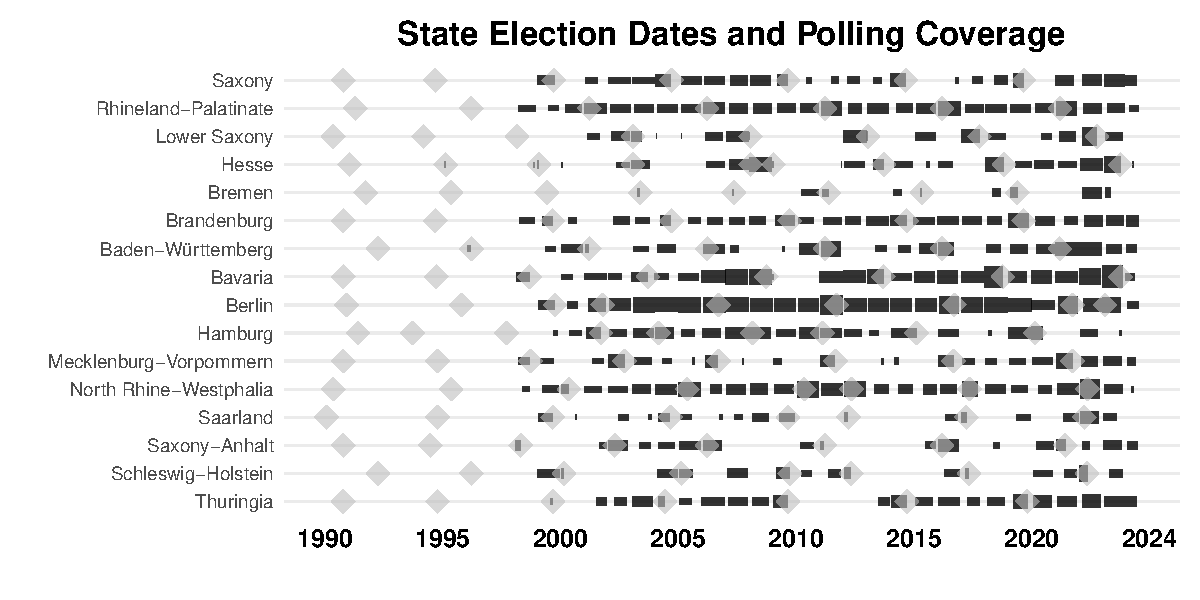
\includegraphics[width=\textwidth]{fg2_polls_coverage_density.pdf}  
    \caption{Poll coverage over time by state. The grey \textcolor{red}{diamonds in the background} represent \textcolor{red}{election dates}. The black segments indicate polling coverage; the larger the segments, the more polling data are available in a given year.}
    \label{fig:polls-coverage}
\end{figure}


\textcolor{red}{For applying the general model, it is crucial to select fundamental predictors relevant to the specific context. In our case, we choose predictor variables commonly used in forecasting models for German federal elections.}  First, government participation is a critical predictor, as incumbency generally confers electoral advantages. Voters often prefer incumbents, based on their perceived competence or continuity in governance~\citep{allers2022parties,eggers_incumbency_2017}.
We add a dummy variable indicating whether a party was part of the state government.  Second, we include a variable that indicates to which party the incumbent prime minister (\textit{Ministerpräsident}) belongs. The incumbent status has been used for forecasting in federal elections~\citep{munzert_2017}. The largest party, typically responsible for government formation, may benefit from strategic voting by citizens seeking to influence future coalition-building processes~\citep{cox1997making,Harsgor2023, Meffert2010}.
% last vote share
The vote share at the last election is an important predictor used previously for forecasting~\citep{munzert_2017, Stoetzer_Neunhoeffer_Gschwend_Munzert_Sternberg_2019} due to the persistent effects of partisan identification on elections~\citep{campbell_impact_1960}. The distribution of such attachments in the aggregate allows us to form expectations about the election outcome under normal circumstances \citep{Converse1966}. For the previous election result (and changes in the polls) we apply the same log-ratio transformation as for the vote shares to ensure they are measured on the same scale.
% new party
We also account for the fact if a party is a new party, defined as those competing in a state for the first time. For instance, this applies to the AfD, which was established in 2015, as well as to our ex-ante forecasts, where the new populist party BSW is anticipated to play a significant role in upcoming elections. Historical data indicate that the AfD has outperformed polling expectations during its initial participation in state elections, a phenomenon consistent with findings that support for radical parties is often underreported in pre-election surveys until they gain parliamentary representation~\citep{valentim_right_2021}.
% Federal trend
Lastly, we include a predictor based on trends in federal polls by applying the dynamic linear model, as we do for state polls. Previous studies report coattail effects, for instance, from the governor vote to related candidates~\citep{MEREDITH_2013}. Coattail effects refer to the influence a popular candidate has on down-ballot races. Furthermore, coattail effects or policy balancing between the federal and state elections have been observed~\citep{BORGES2016104, Kedar2006a}, reinforcing the importance of federal-level trends in state election forecasting.\footnote{\textcolor{red}{In SM~E, we present additional models including variables to account for economic conditions at the time of an election. We include an interaction with government participation of parties as the responsibility for the economic situation might be attributed to the performance of the government~\citep{enns2024understanding, mongrain202110}.}}

\FloatBarrier

\section{\textcolor{red}{Application to German State Elections}}

\subsection{Election Forecasting Model with Varying Lead Times}

To have a reference point for our model, aside from the main model based on polls and fundamentals, we also present a model exclusively based on either polls or fundamentals respectively. The fundamentals-only model can be interpreted as a baseline for the evaluation of our new model; it is based almost entirely on information available immediately after the previous election. Polls capture the latent support for parties over time and allow us to model changes in public opinion between elections. Causally, polls can be seen as following the fundamentals, often capturing the effects of fundamental variables that shape electoral outcomes. For example, the incumbency effect is typically reflected in polls well before an election. 

While our model can generate estimates for any desired time point ahead of an election, we specifically estimate and evaluate it at three key lead times: two months, two weeks, and two days before the election. This approach allows us to assess the model’s performance over time and captures how its accuracy evolves as  election day approaches. By focusing on these intervals, we also cover the most relevant time frames when public attention is particularly high.

\autoref{fig:fundamental-estimates} presents the posterior distributions for the predictors along with their credible intervals. Higher values suggest a stronger influence of the corresponding predictors on the final election outcome.
The \textit{Latent Support}, derived from polling data, stands out as being almost perfectly aligned with the final vote share, highlighting its predictive power. As expected, the influence of \textit{Latent Support} increases as the forecast horizon shortens, indicating that predictions based on recent polling data become increasingly accurate as the election date approaches--with the exception of the model based on fundamentals only because no new information from polls is added.
When combined with the polling data, other fundamental predictors exhibit comparatively minor effects. Among these, the predictors \textit{New Party} and \textit{Prime Minister} are shown to have the largest impact, though their influence diminishes over time as more variance is accounted for by polling data.
In the fundamentals-only model, we observe a persistent negative effect for the \textit{Government Party}, while the predictors \textit{New Party} and \textit{Vote Share Last Election} show substantial effects throughout the forecast period.

The models which include latent support become more precise over time, as indicated by the estimates of the error variance (\textit{Sigma}) for the two models. The error variance is higher two months before the election than it is two weeks before, and higher two weeks before than two days prior. Furthermore, the error variance estimates show that the models incorporating polls have smaller variances compared to the fundamentals-only models, which, interestingly, does not change over time. The temporal consistency of the error variance suggests that the precision of the fundamentals-only model remains relatively constant, regardless of lead time.

In summary, the results of our polling-only model show stronger effects compared to the fundamentals-only model, particularly as election day approaches. This reinforces the idea that the latent support of parties evident in the polls are a consequence of the fundamentals, capturing their effects over time.


\begin{figure}[!t]
    \centering
    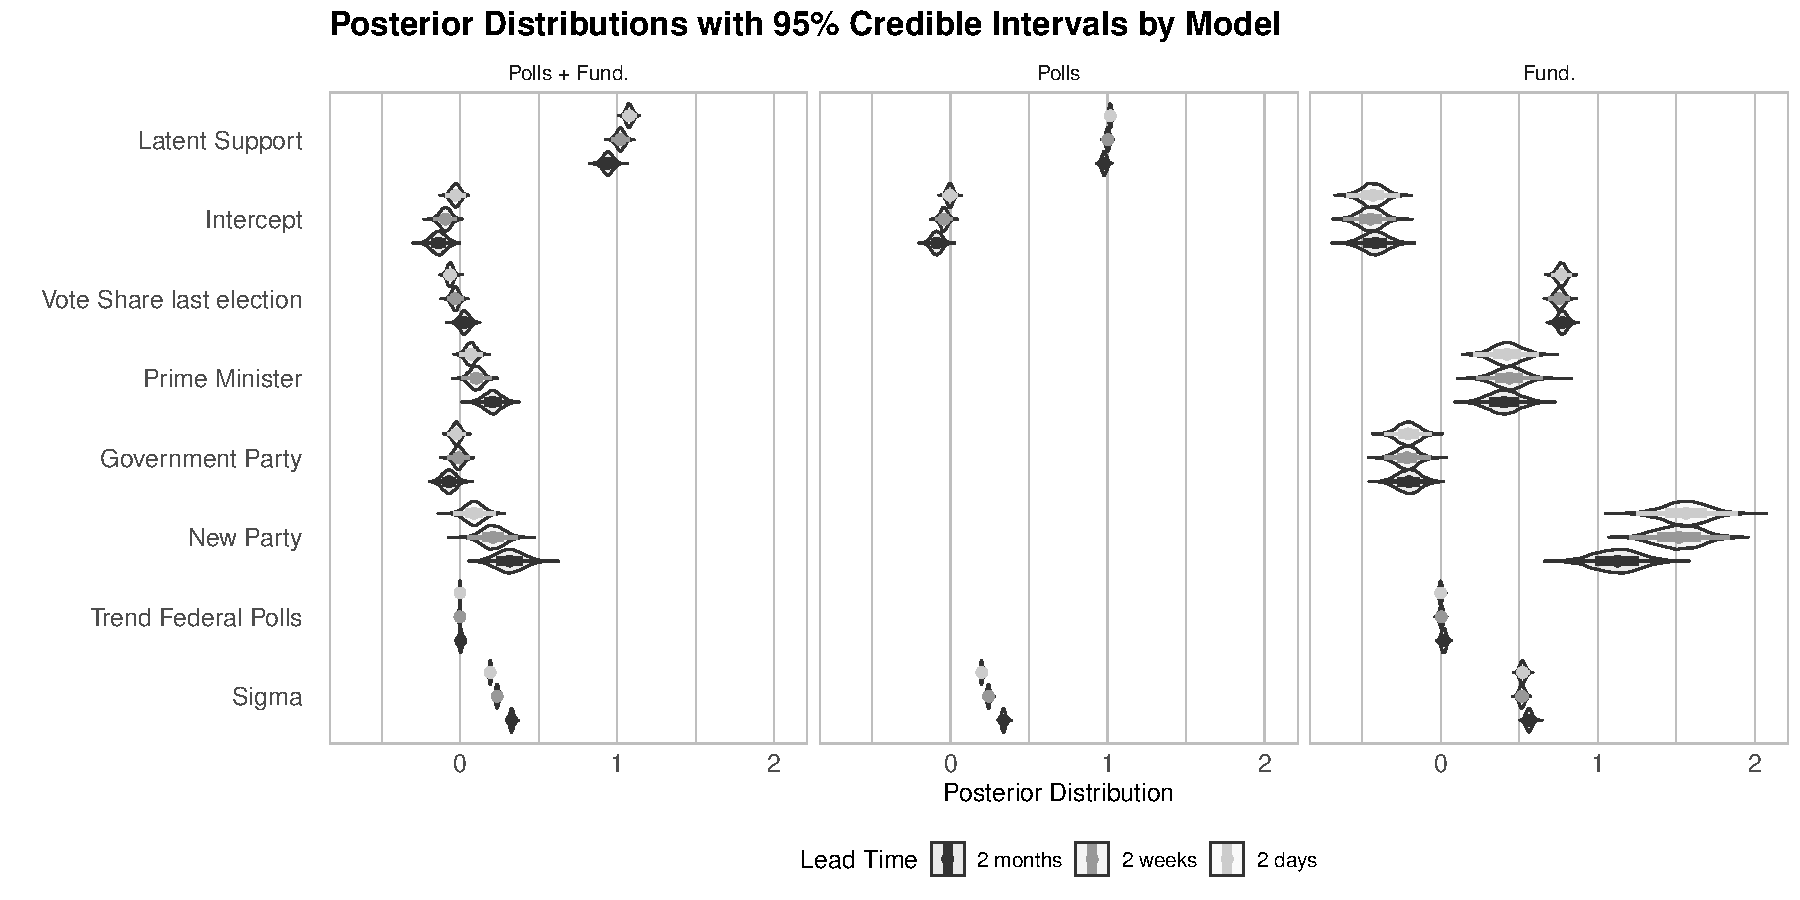
\includegraphics[width=\textwidth]{fg3_fig_eval_bayes_par.pdf}  
    \caption{Posterior distributions for the predictors along with their credible intervals across models.}
    \label{fig:fundamental-estimates}
\end{figure}

\FloatBarrier
\subsection{Evaluation Based on Past Elections}
\FloatBarrier


We evaluated the performance of our model using historical state election results from 2010 to 2023 for all major parties. \autoref{fig:model-evaluation-mae} shows the Mean Absolute Error (MAE)\footnote{For comparison with other studies, we also provide the Root Mean Square Error (RMSE) in SM~C.}. Across three different lead times, the model that combines both fundamentals and latent polling support consistently performs best. Two months before the election, this model achieves an MAE of 3.09pp. As the election approaches, the accuracy improves, with the MAE decreasing to 2.19pp two weeks before the election and further to 1.46pp two days before the election. This is a very accurate forecast, getting very close to the final result.

The results further underscore the importance of polling information for forecasting. A model that incorporates latent polling support consistently outperforms a fundamentals-only model across all specified lead times. While fundamentals offer valuable insights early in the election cycle, their impact diminishes as polling data becomes more available. This finding highlights that, even in subnational elections, pre-election polls are the most reliable tool for forecasting outcomes in the immediate lead-up to election day.

\textcolor{red}{Our evaluation shows that the performance of the model is comparable to, and in some cases better than, other established election forecasting models. For instance, \citet{jennings2018election} report an MAE of 2.7pp for presidential elections and 1.8pp for legislative elections, with performance varying based on the electoral system. In single-member district (SMD) systems, the MAE tends to be higher (2.3pp), whereas proportional representation systems have lower MAEs (1.6pp). Our model's performance is in line with these findings, particularly at the two-week and two-day lead times.}

\textcolor{red}{Similarly, \citet{shirani2018disentangling} found a survey error, measured by root mean square error (RMSE), of approximately 3.5pp, about twice the size of the margins of error typically reported by polling organizations. In contrast, our model achieves much smaller errors when using a model that combines polling and fundamentals, where the RMSE improves to up to 2.06pp two days prior to the election.}

\textcolor{red}{A direct comparison to forecasts for German federal elections shows that our model also performs well. \citet{munzert_2017} found that the RMSE for structural models in German federal elections ranged from 2.54pp to 1.98pp, depending on the proximity to election day. In the last few days before the election, models that include polling data showed substantial improvements, with the RMSE shrinking to as low as 1.69pp. Our model, similarly, improves substantially as the election approaches having an RMSE of 2.06pp two days before the election, comparable to the national election forecast.}

Our model also produces credible 5/6 intervals that provide a reliable measure of forecast uncertainty. The 5/6 credible intervals from the full model consistently cover the true election outcomes around 83 \% of the time. In the applied section below, we describe the coverage of credible intervals for our forecast of three state elections.

\begin{figure}[t!]
    \centering
    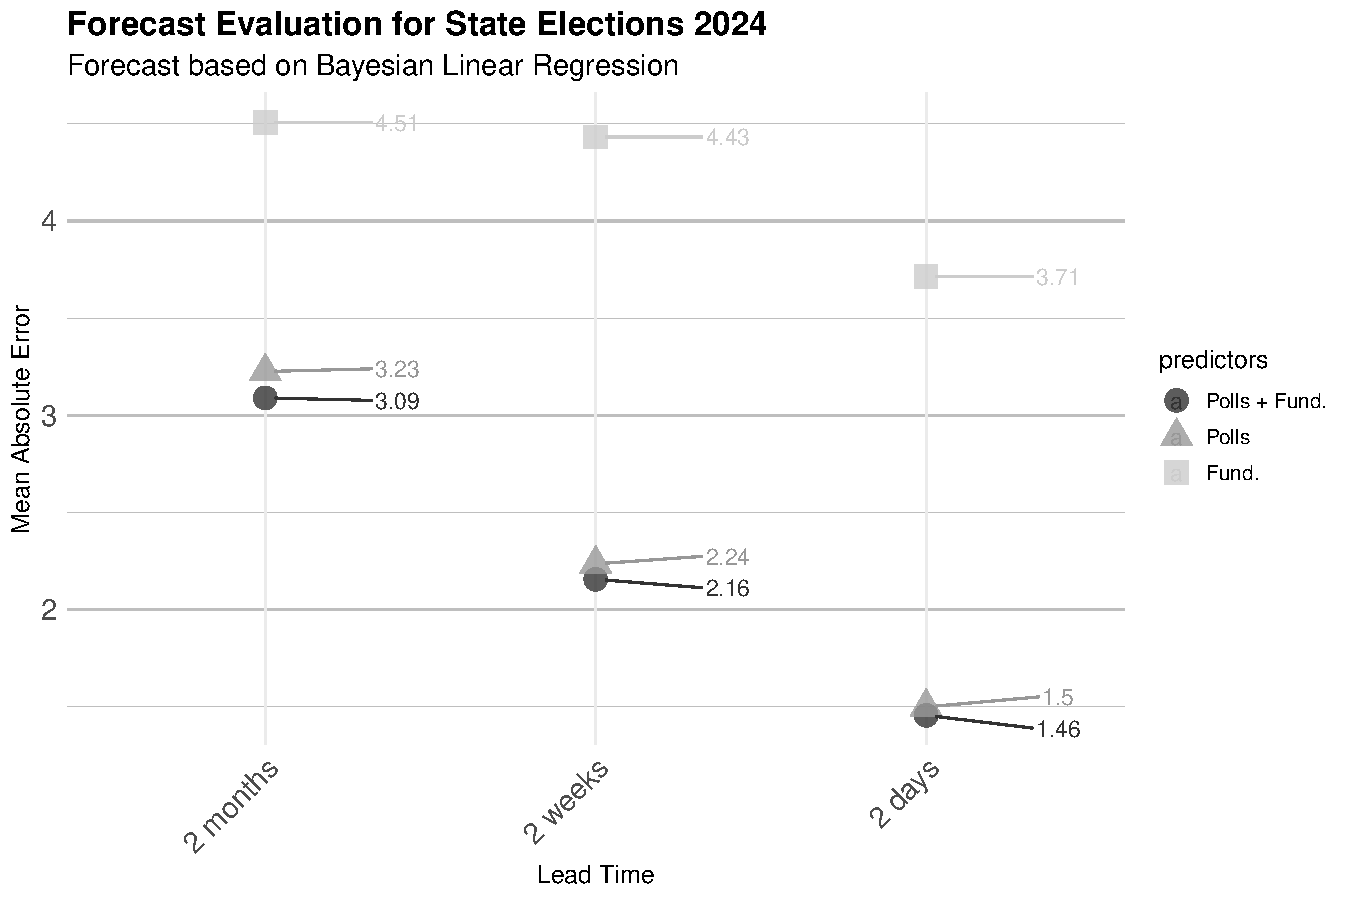
\includegraphics[width=\textwidth]{fg4_fig_eval_bayes_mae-2.pdf}
    \caption{Mean Absolute Error (MAE) for the state elections from 2015 to 2023, comparing different model specifications. The MAE values are calculated for forecasting models using different lead time (days, weeks, and months) prior to the election. This figure demonstrates the accuracy of the model's predictions over time, with lower MAE values indicating better model performance.}
    \label{fig:model-evaluation-mae}
\end{figure}




\subsection{Ex-ante Forecast of the 2024 State Elections}



We forecast the state elections in three German states: Saxony and Thuringia on 1 September 2024 as well as Brandenburg on 22 September 2024\footnote{These forecasts were preregistered (OMITTED).} %~\citep{stoetzer_erfort_preregistration_2024a,stoetzer_erfort_preregistration_2024}.}. 
Although all three states are located in East Germany, they exhibit distinct political landscapes leading up to these elections. Both Brandenburg and Saxony are governed by coalitions comprising the SPD, CDU, and Greens. However, while Brandenburg's prime minister is a Social Democrat (SPD), Saxony's government is led by the CDU. Thuringia presents a more complex situation, with a minority government formed by the Linke, SPD, and Greens, and tolerated by the CDU. Notably, Thuringia is the only state with a Linke head of government in Germany. In all three states, the radical-right AfD has made gains in the polls since the last elections. Moreover, surveys indicate that the newly founded BSW party, which largely consists of former Linke members, was expected to win more than 15\% of the vote.

\autoref{fig:all-forecasts} displays our ex-ante forecasts for the three state elections in 2024, made at two months, two weeks, and two days before the election. The columns in the subplots correspond to the full model (combining fundamentals and polls), the polls-only model, and the fundamentals-only model. Separate plots showing the forecasts from the hybrid model are available in SM~B. 

\begin{figure}[!t]
    \centering
    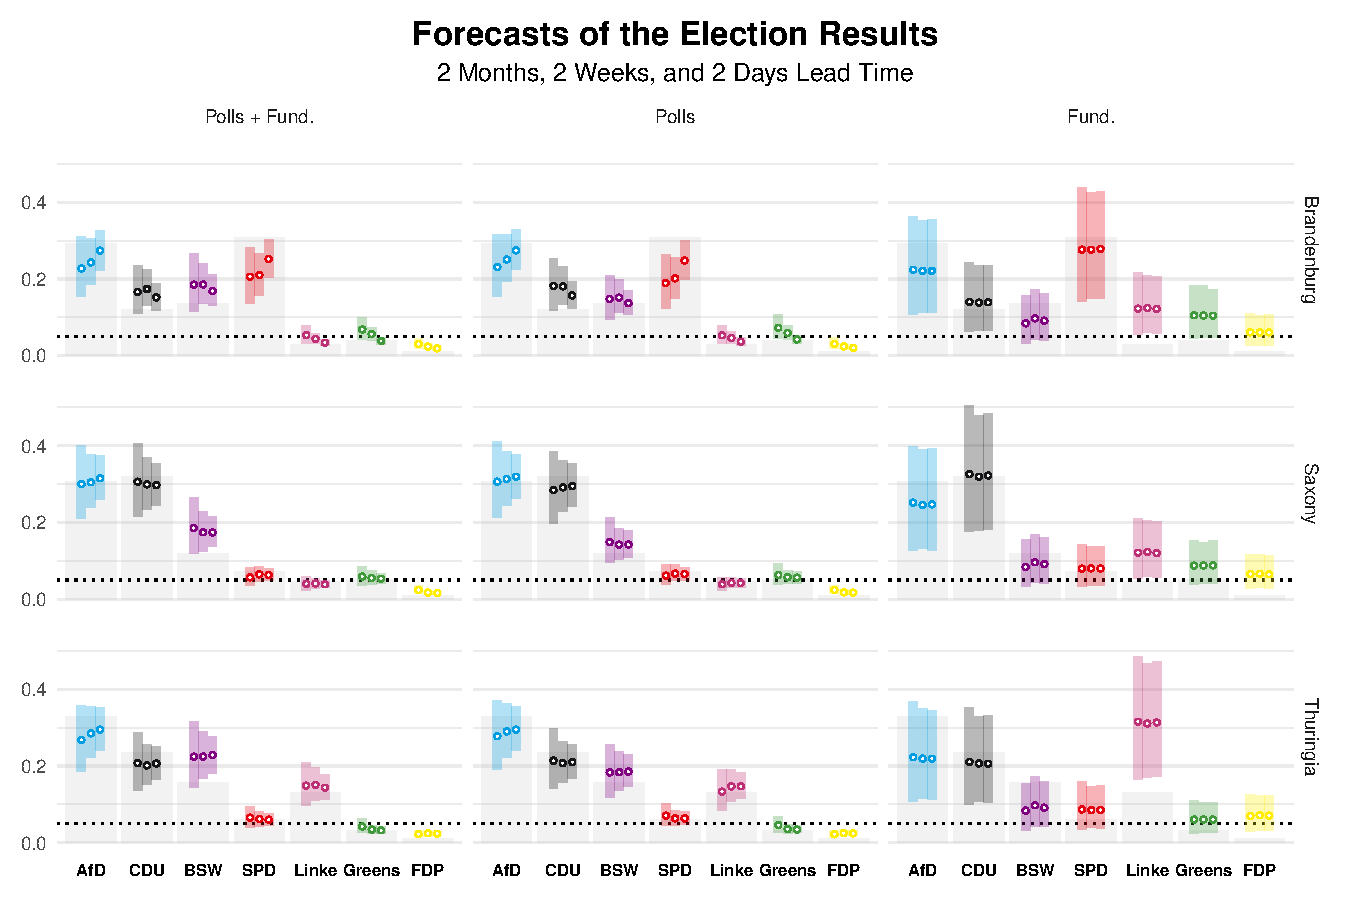
\includegraphics[width=\textwidth]{fg5_all_fcsts.pdf}
    \caption{Ex-ante election forecasts for the 2024 state elections in Brandenburg, Saxony, and Thuringia at two months, two weeks, and two days before the election, grouped from left to right. Points represent the forecasted vote shares for each party, with the intervals showing the 5/6 credible intervals. The grey bars in the background represent the actual election outcomes.}
    \label{fig:all-forecasts}
\end{figure}

When interpreting the forecasts, it becomes evident that the hybrid model and the polls-only model produce similar results. However, the inclusion of fundamentals appears to bias towards new parties, giving them a slight bonus compared to models based exclusively on polls. Comparing our forecasts to the actual election results, we find that the full model overestimated BSW's vote share while underestimating the other parties. This overestimation may stem from the fact that the “new party bonus”, which benefited the AfD as a newcomer only years before, did not translate to BSW. One plausible explanation is that surveys may have been biased against the AfD due to its radical-right positioning, an effect which was not observed in the case of the  BSW~\citep{valentim_right_2021}.

The fundamentals-only model significantly overestimated the Linke, as it primarily relies on historical vote shares, overlooking polls which predicted a substantial defeat for the party. In this model, BSW's vote share remains greater than zero due to the 'new party bonus' discussed above.

As the election nears, we observe a consistently decreasing forecast uncertainty, evidenced by shrinking credible intervals. However, when relying solely on fundamentals, the credible intervals remain wider and do not narrow significantly — a predictable outcome given that polling data helps reduce forecast uncertainty, especially closer to the election date.

Our model also allows for the calculation of probabilities associated with key political events. For instance, two weeks before the election in Saxony, the probability that the CDU would become the strongest party stood at 47.8\%, while the probability that the incumbent CDU-SPD-Greens coalition would secure a majority was only 13.3\%. Similarly, in Brandenburg, the probability of a majority for the incumbent SPD-CDU-Greens coalition was estimated at 34\%.

Overall, the model's forecasts performed well with a Mean Absolute Error (MAE)\footnote{For comparison with other studies, the Root Mean Square Error (RMSE) is provided in SM~D.} of 3.16~pp across all states and parties, two months before the election. As expected, forecast errors decreased as the election approached. Two weeks before the election, the MAE had dropped to 2.74~pp, and two days before, the MAE further decreased to 2.03~pp. Both the hybrid model and the polls-only model performed well. Errors for the polls-only model range between 1.61~pp two days and 2.73~pp two months before the election, comparable to federal election forecasts. In contrast, forecasts for Thuringia showed greater errors, particularly in the fundamentals-only model, where the mean error exceeded 7~pp due to more substantial electoral shifts.

Regarding the 5/6 credible intervals, the full model forecasts for the 2024 state elections correctly predicted outcomes slightly less than 5 out of 6 times, with an accuracy of 67\% two months before the election, 57\% two weeks before, and 71\% two days before. Forecasts from the polls-only model were within the credible intervals more frequently, achieving 6 pp higher accuracy rates on average. In contrast, the fundamentals-only model had an accuracy equal to the hybrid model; note, however, that the model's credible intervals are also much wider.


\begin{figure}
    \centering
    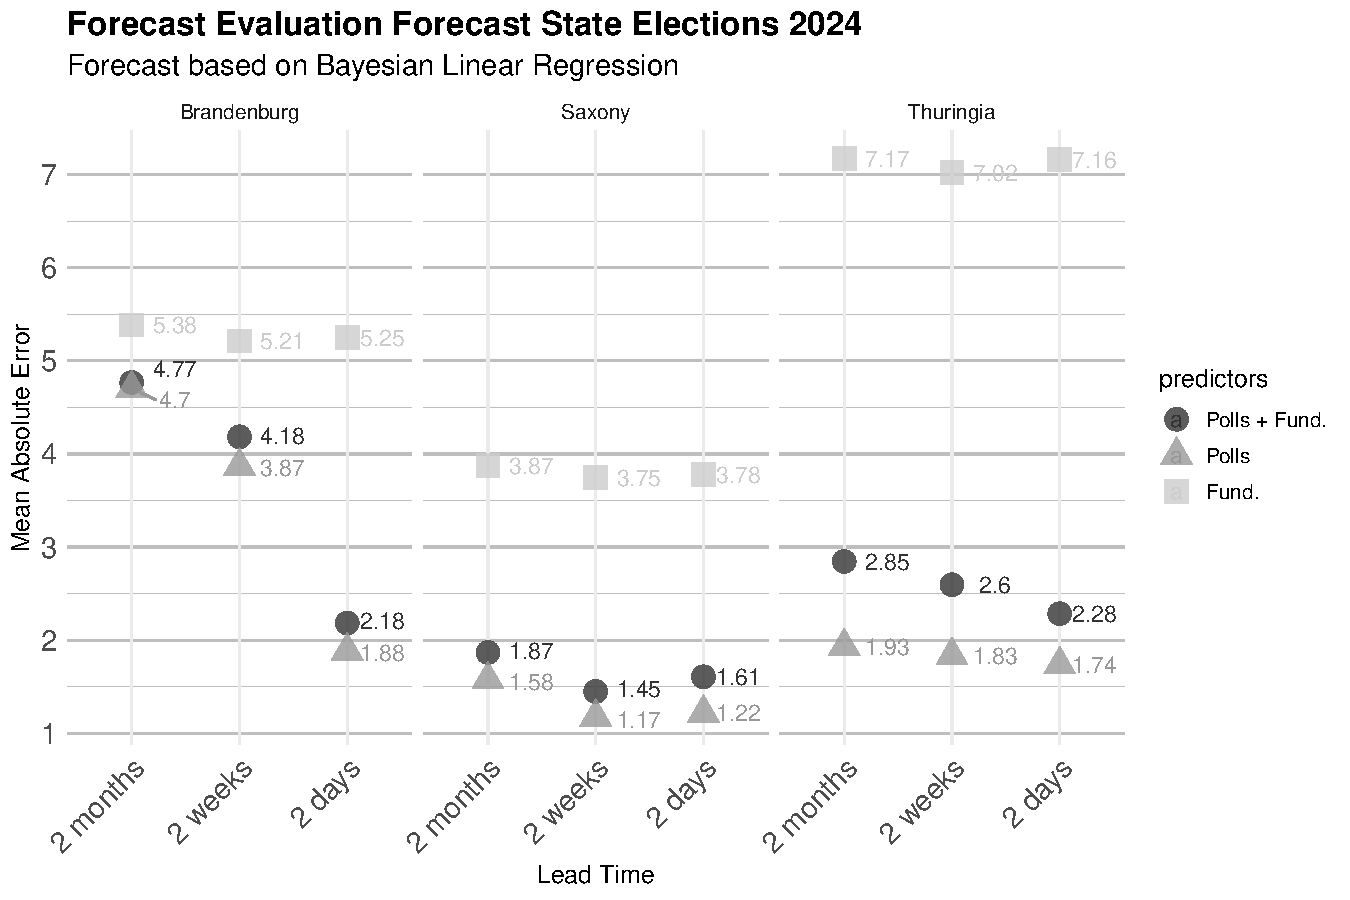
\includegraphics[width=\textwidth]{fg6_forecast_evaluation_mae.pdf}
    \caption{Mean Absolute Error (MAE) for the ex-ante forecasts of the 2024 state elections, comparing different model specifications. The MAE values are calculated for forecasting models at different time points (days, weeks, and months) before the election. This figure highlights the improving accuracy of the forecasts as the election approaches, with lower MAE values reflecting better model performance.}
    \label{fig:forecast-evaluation-mae}
\end{figure}

\FloatBarrier
\section{Discussion}

Are subnational election outcomes predictable? At times, dramatic shifts between parties occur which seem fundamentally unpredictable -- for example, the unprecedented success of the Greens in the 2011 state election in Baden-Württemberg just days after the Fukushima nuclear accident, which had a long-lasting impact on the local party system. Other elections at sub-national level seem to be characterized by unshakable stability -- such as the CSU's decades-long dominance in state elections in Bavaria. In a similar vein, subnational election results impact national politics, such as in 2005, when the then Chancellor Schröder called an early federal election on the evening of the Social Democrats' defeat in the state election in North Rhine-Westphalia, which, in turn, heralded the end of the red-green federal government. 

Despite their significant relevance in multi-level systems, subnational elections have been relatively understudied using forecasting models. Instead, the forecasting literature has primarily focused on national elections. Developing effective forecasting models for subnational elections offers valuable insights into electoral behavior at the regional level, especially when data is scarce or elections are highly localized. This paper presents a forecasting model combining polling data and fundamentals to predict election outcomes. The model was tested on German state elections from 1990 to 2024, achieving notable accuracy across different lead times. The results show that the hybrid polls-and-fundamentals model consistently outperforms models based purely on polling or fundamentals, with a mean absolute error (MAE) ranging from 1.46pp two days before the election to 3.09pp two months before. Ex-ante forecasts for a set of three 2024 elections also performed well, further validating the model's utility in subnational election forecasting.

\textcolor{red}{The potential for applying this model to other subnational election contexts, outside of Germany, is promising. The consistent performance across different German states suggests that similar models could be adapted for federal or regional elections in other countries with comparable political structures. Many federal democratic systems feature subnational elections that shape regional governance and national politics. Comparable cases include Canada (provincial elections), Switzerland (cantonal elections), and Spain (autonomous community elections), where multi-party competition and varying polling availability present similar forecasting challenges. While the model could, in principle, be applied to national elections, existing approaches at that level already provide well-established forecasting methods. Our contribution lies in adapting and refining these techniques for subnational elections, where forecasting models remain underdeveloped, and our results demonstrate that the theoretical and methodological foundations perform well in this context.}

\textcolor{red}{Looking ahead, there are several ways to extend and refine the model. Alternative modeling approaches, such as Seemingly Unrelated Regression (SUR) and Dirichlet regression, could be explored in future research. The SUR model allows for correlated errors across party forecasts, which may be useful in some election forecasting contexts~\citep[see e.g.,][]{mongrain202110}. However, it may also require election-specific covariance structures, as different parties compete in different elections, making estimation challenging with limited data. Similarly, Dirichlet regression models are designed for compositional data and can account for the fact that vote shares sum to 100\%~\citep[see e.g.,][]{hanretty2021forecasting, Stoetzer_Neunhoeffer_Gschwend_Munzert_Sternberg_2019}. Based on our experience with Dirichlet forecasting models, we have often found transformations of the dependent variable, such as the log-ratio approach used here, to be more practical, but future research might prove otherwise.}

Another promising extension would be to integrate the latent support model directly into the forecast estimation process. By incorporating the uncertainty associated with latent support estimates into the overall forecast, the model could provide more accurate uncertainty intervals, offering a more nuanced understanding of forecast reliability, especially when polling data are sparse or less consistent. 

In conclusion, the model presented here demonstrates strong potential for forecasting subnational elections with high accuracy, and with further refinements, it could become an even more robust tool for electoral forecasting in various contexts.




\end{doublespacing}





\newpage
\bibliographystyle{plainnat}  % Use a style compatible with natbib
\bibliography{references.bib}


\clearpage

\newpage
\appendix

\textbf{Declaration of generative AI and AI-assisted technologies in the writing process}. During the preparation of this work the authors used ChatGPT 4o in order to copy-edit written paragraphs of text. After using this tool/service, the authors reviewed and edited the content as needed and take full responsibility for the content of the publication.


\end{document}


